\subsection{Analyzing and Extracting Functions from PLC Firmware}
\label{sec:plc}

In this section, we demonstrate our ability to analyze continuous equation models of the firmware of a PLC (Fig.~\ref{fig:plc-stats}).
We recovered the following core model from the firmware's PID (proportional-integral-derivative) functions, where I and D are uninterpreted functions for integral and derivative, respectively:
\begin{equation}
v_{6}(
(v_{3}-v_{2})+
\frac{1}{v_{5}}
I(v_{3}-v_{2},1000t)
+
v_{1}
D(v_{3}-v_{2},1000t)
)+v_{0}+v_{7}
    \label{eqn:ideal_pid_fixcycle}
\end{equation}

For analysis in Matlab, we needed to also take into account some non-infinitesimal measure of time.
We simplified the recovered equation further via a few additional common axioms, e.g. $new\_sym = v_{3} - v_{2}$, $integ\_e\_dt = I(binds_{i0}, binds_{i1})$:
\begin{equation}
    K_{p}(
        e + 
        \frac{1}{\tau_{i}}
        \int e \mathrm{d}t
        + 
        \tau_{d}
        dv e t
    ) + b
    \label{eqn:ideal_pid_fixcycle}
\end{equation}

Eqn.~\ref{eqn:ideal_pid_fixcycle} more closely matches the traditional PID formulation, where $K_{p}$ is the proportional gain constant the ICSREF attack modified.
The other equations InteGreat\ recovered from the PLC did not require further constructed abstraction specifications.

\textbf{Discovering Additional Hardware.}
In the lifted version of the firmware, we also found an obscure scaling was applied to the sensor value for the input reactor pressure before it was supplied to Eqn.~\ref{eqn:ideal_pid_fixcycle}:

\begin{equation}
    P = 1000(((P_{digital} / 30000) - 0.0046) / 0.9876) + 2000
	\label{eqn:input-conv}
\end{equation}

\begin{figure*}
    \centering
    \begin{subfigure}[b]{0.49\textwidth}
        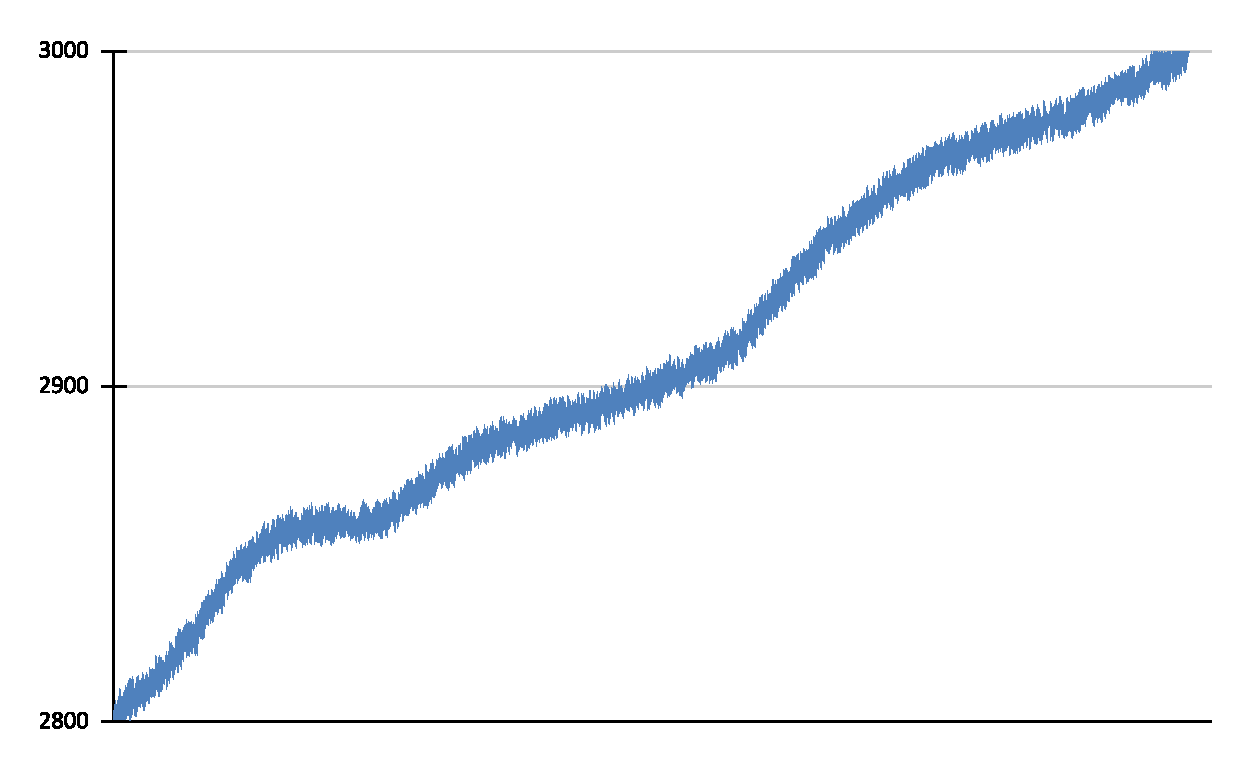
\includegraphics[width=\textwidth]{fig/plc-orig.pdf}
        \caption{Naive Attack Reproduction}
        \label{fig:orig-attack}
    \end{subfigure}
    \hfill
    \begin{subfigure}[b]{0.49\textwidth}
        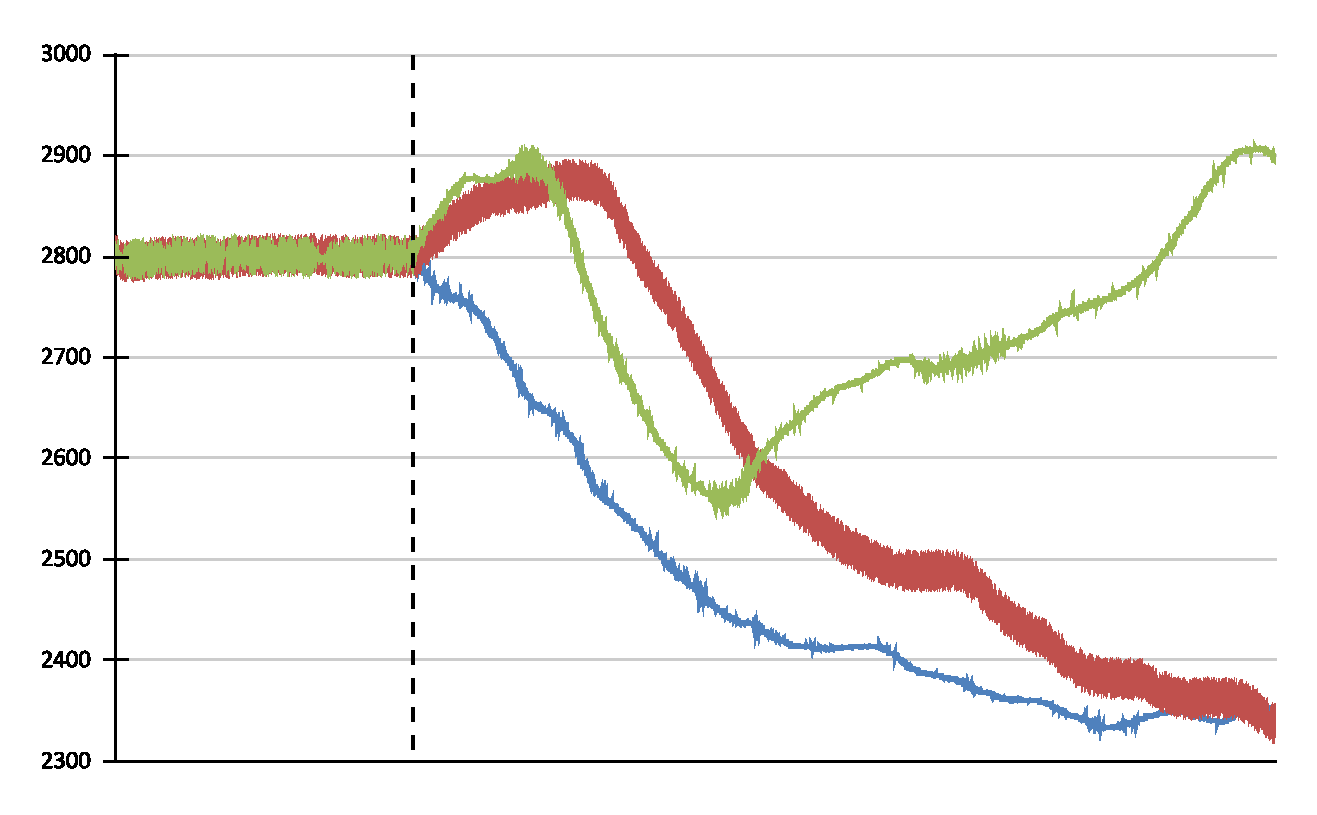
\includegraphics[width=\textwidth]{fig/dashed-plc.pdf}
	    \caption{Voltage Corrected Destabilization}
        \label{fig:noconv-attack}
    \end{subfigure}
    \hfill
	\caption{\textbf{Left}: An attempt to stage the ICSREF attack using the recovered model without taking into account the physical effects of digital-to-analog conversion. The plant shuts down upon when the reactor pressure hits 3000 kPa. \textbf{Right}: Variations of the staged attack with physical effects accounted for. The dashed line is the point at which the attack occurs (the 4 hour mark).}
    \label{fig:plc-eval}
\end{figure*}

We also were recovering the wrong value for the reactor pressure when we staged normal operation of the environmental model using our lifted equations, depicted in Fig.~\ref{fig:orig-attack}.
This led us to discover the reactor pressure (which starts at 2800 kPa in the TE simulation) was supplied to the PLC through a \emph{physical wire} connected to a separate Analog-to-Digital Converter (ADC), rather than a serial port.
The original pressure value is converted to a voltage value between 1 and 3, and then this voltage is converted back to a digital value on the physical PLC (30,000) corresponding to 3 volts.

We confirmed this was the case with the ICSREF authors.
Because of the the physical effects of the ADC being taken into account, the scaling equations applied to PLC I/O values in the Matlab environmental model used by the paper were \emph{not} the inverse of Eqn.~\ref{eqn:input-conv}.
Instead, the Matlab environmental model had no scaling to account for the ADC and the firmware \emph{implicitly} suggested the ADC was present via the scaling computation.

Even without ground truth, we were able to discover the presence of a physical ADC by analyzing a firmware's equations after lifting.
This demonstrates novel discoveries about a system's environment can be made by using InteGreat\ to analyze firmware.

\section{Precise Destabilization Attack Development}
The ICSREF attack flipped the sign on the proportional gain constant of the first of the firmware's PID calls.
By recovering the continuous equations the firmware image implemented, we were able to \emph{stage} this attack without access to the physical PLC.

A naive extraction of the firmware's implementation into Matlab, maintaining the original voltage conversions discussed above, results in Fig.~\ref{fig:orig-attack} when staging the attack.
This is because  the input and output values to the PLC's equations are affected by the scaling decided by the physical digital-to-analog and analog-to-digital converters.
This proposes the importance of a hybrid approach to modeling in the current domain of firmware rehosting~\cite{jetset,p2im,halucinator}.
While an exact emulation of the firmware's operation is desirable for dynamic analysis and testing (e.g. fuzzing), it is also necessary to verify that the I/O boundaries of the system are consistent with the physical environment or environmental model the emulation is attached to.

Moving forward with this understanding, we were then able to correctly reproduce the destabilizing effects on reactor pressure created by uploading code to the PLC (Fig.~\ref{fig:noconv-attack}).
\textbf{Red} represents the original PLC firmware behavior from the ICSREF paper.
However, notice that the paper included an unexplained positive bump at the point of attack.
Lifted equations allow us to explore an idealized model of the firmware's implementation: by removing all scaling operations from Matlab and the recovered model, we attained the line in \textbf{Blue}.
In doing so, we discovered exactly how much the ADC voltage conversion affects the cyberphysical system's dynamics.
The \textbf{Green} line represents a case where the attack \emph{did not} occur but control over the reactor pressure is given to the PLC (with ADC scaling).
This scaling makes the pressure of the plant far less stable, a feature of the system not addressed in the original ICSREF paper.

As the above evaluation demonstrates, using InteGreat\ we were able to both reproduce and verify the existing \emph{ICSREF} attack on a PLC and extend it to target an arbitrary reactor pressure levels by modifying the proportional gain constant in the recovered model to desired values.
The recovered equations were of value in \emph{precisely} destabilizing the plant's reactor pressure while maintaining the appearance of correct behavior, similar to stuxnet~\cite{baezner2017stuxnet}.
Because the recovered models of the PLC's control equations are general, it was also possible to experiment with any variety of potential modifications to the PID controller and explore a variety of reachable states given the environmental model.

\section{Discussion}

Informed by both the Jetset and Edact-Ray works, InteGreat adopts an opinionated perspective on the challenges facing binary program analysis.
It attempts to address universal and necessary limitations to abstract interpretation, such as the modeling of microarchitectural semantics and state explosion, by applying the well-worn technique of wrapping these complexities in a layer of indirection, and then automates the construction of this indirection.
While this alleviates the \emph{immediate} difficulties involved in inferring loop invariants and pointer analysis, InteGreat also has the explicit limitation of requiring users to leave these semantics undefined or provide their own formulae for resolution.

We therefore consider a primary future application of InteGreat being \emph{lifting libraries}.
By incorporating an object-oriented approach for abstraction specifications, the InteGreat framework is able to continually expand its base of knowledge.
A given set of lifting rules can be written and then shared, similar to a library, for the analysis of wide ranges of firmware binaries.
These libraries may also be generated via automated methods, and serve as a compressed encoding of more complex inference procedures.
Moreover, because it is possible to encode uniform semantics for a given system, these libraries can begin to function as ``contracts'' to ensure a system meets certain regulatory implementation requirements, something top-down verification cannot provide.

InteGreat does not solve the \emph{internal} or \emph{external} semantic problems posed in Section~\ref{sec:jetset-limitations} or the more general problem of missing information in a system's specification.
Instead, the system attempts to provide a better interface for management of this problems.
It does so by making no assumptions about the underlying semantics of the system, building a model of the system from the ground up by starting with the implementation, rather than a mathematical model.

In providing an interface for a more abstract representation the system during symbolic execution, InteGreat is able to rely on additional input for undefined or undecidable cases and extract useful models in cases where no such additional information is required or feasible to provide.
InteGreat thereby alleviates the need to treat complex systems as complete black-boxes,\footnote{The dangers of making representational assumptions were demonstrated in Chapter~\ref{chap:info}.} and instead attempts to restrict the use of black-boxes to cases where information on the system is legitimately missing.
